Die bisherige Herangehensweise, den Niederschlag über das Jahresmittel zu Evaluieren ist nicht hinreichend genau. Dadurch wird die lokale und vor allem zeitliche Varianz zu stark beeinträchtigt. Laut D.Maraun \cite{biasMaraun} ist dafür ein Herangehensweise über stochastische Quantile-Mapping nötig.
\section{Herangehensweise}
\begin{itemize}
	\item Berechnung des 99. jährlichen Quantils aller Datensätze
	\item Vergleichen dieses Quantils mit dem Quantil der Beobachtungsdaten.
	\item Zur Besseren Darstellung Mitteln über die Differenzen aller Jahre
\end{itemize}

\section{Differenzen des 99. Quantils}
Von den Datensätzen (historical, evaluation und APGD) wurden zunächst das jährliche 99. Quantil berechnet. Von den Modelldaten wurden wie oben die Beobachtungsdaten abgezogen. Um eine einfachere Darstellung der Ergebnisse zu gewährleisten wurde über Differenzen aller Jahre gemittelt. Es ergab sich die Grafik in Abb. \ref{fig:quantile_all}. Wie darin zu erkennen ist, ist im Mittel kaum noch ein Unterschied zwischen den 99.Quantilen zu erkennen. Die Kurve zieht sich für alle Datensätze  gleich, auch die Anzahl der Abweichungen sind ähnlich. Um dieses Ergebnis zu unterstreichen wurden noch die dazugehörigen Boxplots in Abb.\ref{fig:quantile_all_boxplots} abgebildet: Man erkennt, dass die Biases kaum noch variieren. Dies spricht dafür, dass die Extremniederschläge stark unterschätzt werden. Dies gilt für beide Klimamodelle, CORDEX FPS-CPS (ALP-3) und CLMcom-CCLM4-8-17 (EUR-11). Dieses Verhalten zeigt sich über alle Jahren(vgl. dazu Abb. \ref{fig:quantile_alp3}): das Mitteln hat nicht viel der Variabilität gekostet und somit reicht die Darstellung der gemittelten Daten aus, um diese Auswirkung des Modells abzubilden. Beachtenswert in den Grafiken von Abb.\ref{fig:quantile_alp3} ist, dass sich die maximalen Abweichungen nun auf zwei Hauptspots reduzieren, die im Süden des Alpenhauptkamms und bei Genua liegen. 
\begin{figure}
	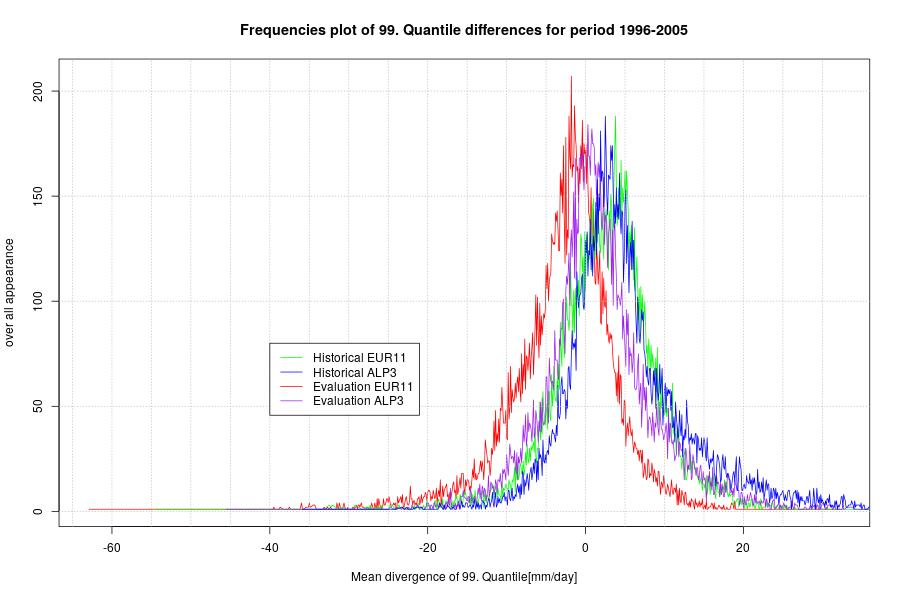
\includegraphics[width=0.8\textwidth]{quantile_all/freq_mean_q99.jpg}
	\caption{Die Abweichungen vom 99. Quantil des Niederschlags, gemittelt über alle Jahre}
	\label{fig:quantile_all}
\end{figure}
\begin{figure}
	\begin{subfigure}{0.49\textwidth}
		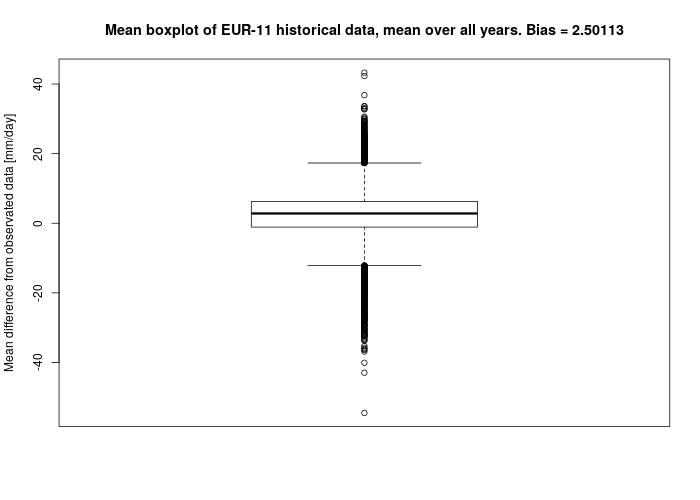
\includegraphics[width=\textwidth]{quantile_all/mean_q99_boxplot_hist_eur11.jpg}
		\caption{EUR-11, Historical}
	\end{subfigure}
	\begin{subfigure}{0.49\textwidth}
		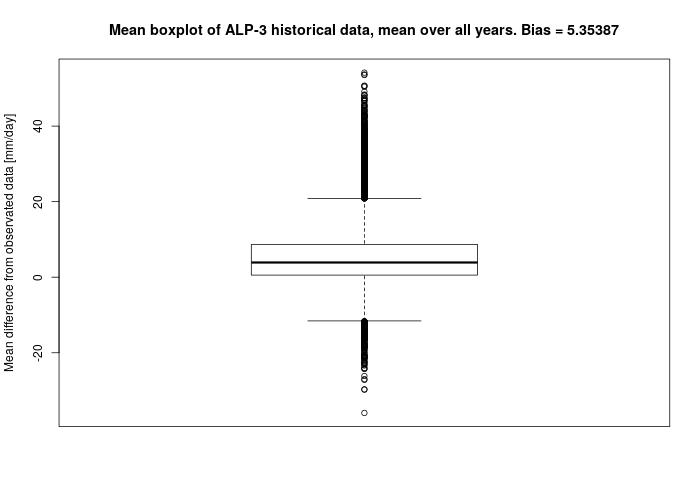
\includegraphics[width=\textwidth]{quantile_all/mean_q99_boxplot_hist_alp3.jpg}
		\caption{ALP-3, Historical}
	\end{subfigure}
	\begin{subfigure}{0.49\textwidth}
		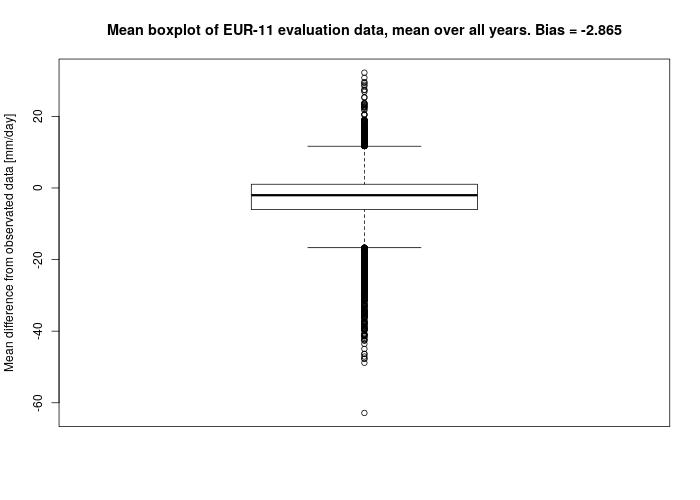
\includegraphics[width=\textwidth]{quantile_all/mean_q99_boxplot_eval_eur11.jpg}
		\caption{EUR-11, Evaluation}
	\end{subfigure}
	\begin{subfigure}{0.49\textwidth}
		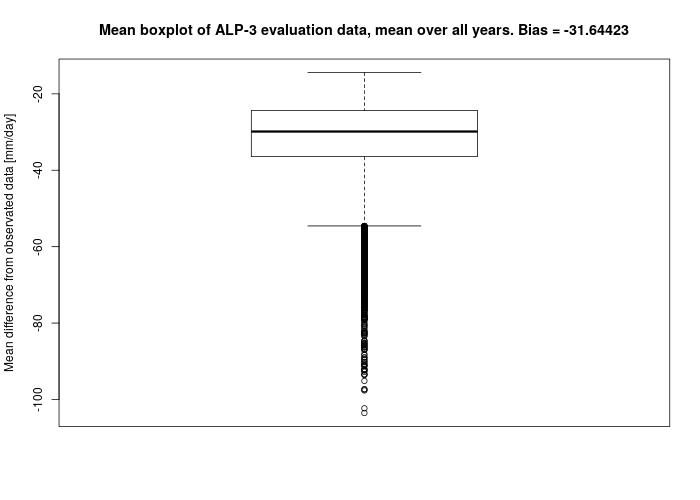
\includegraphics[width=\textwidth]{quantile_all/mean_q99_boxplot_eval_alp3.jpg}
		\caption{ALP-3, Evaluation}
	\end{subfigure}
	\caption{Boxplots der Abweichungen im 99.Quantil, gemittelt über alle Jahre für die 4 Datensätze.}
	\label{fig:quantile_all_boxplots}
\end{figure}
\begin{figure}
	\begin{subfigure}{0.32\textwidth}
		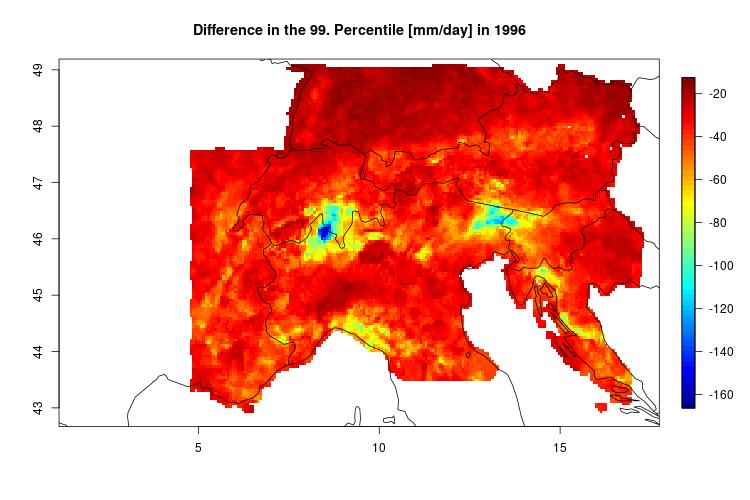
\includegraphics[width=\textwidth]{quantile_all/1996dif_q99_hist_eur11.jpg}
		\caption{Historical, EUR-11, 1996}
	\end{subfigure}
	\begin{subfigure}{0.32\textwidth}
		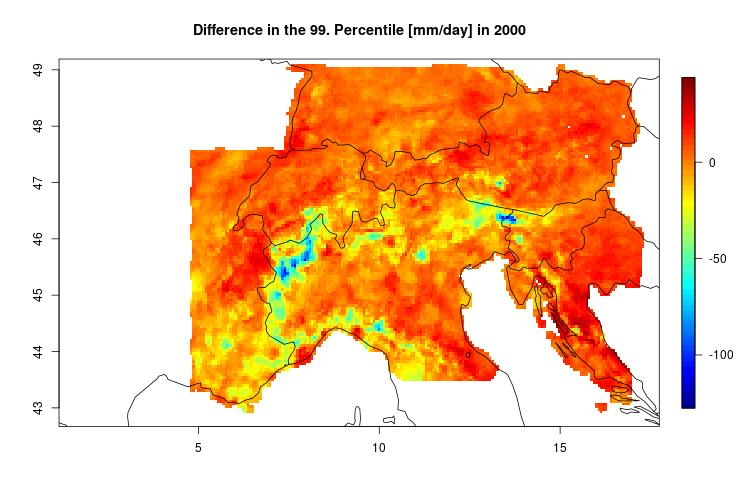
\includegraphics[width=\textwidth]{quantile_all/2000dif_q99_hist_eur11.jpg}
		\caption{Historical, EUR-11, 2000}
	\end{subfigure}
	\begin{subfigure}{0.32\textwidth}
		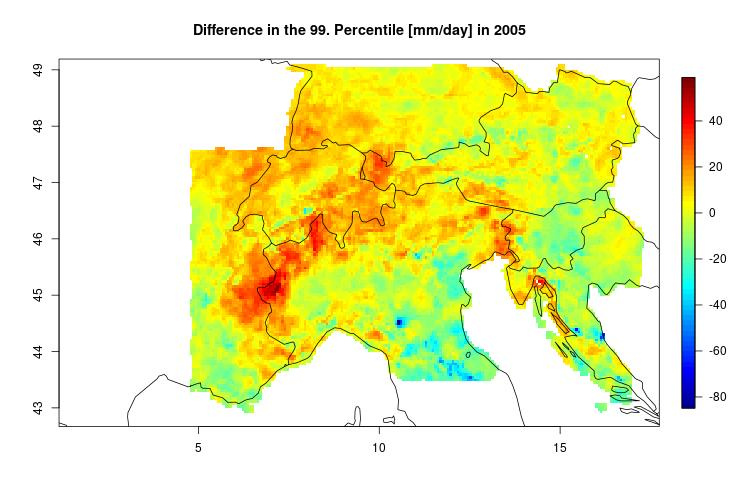
\includegraphics[width=\textwidth]{quantile_all/2005dif_q99_hist_eur11.jpg}
		\caption{Historical, EUR-11, 2005}
	\end{subfigure}
	\begin{subfigure}{0.32\textwidth}
		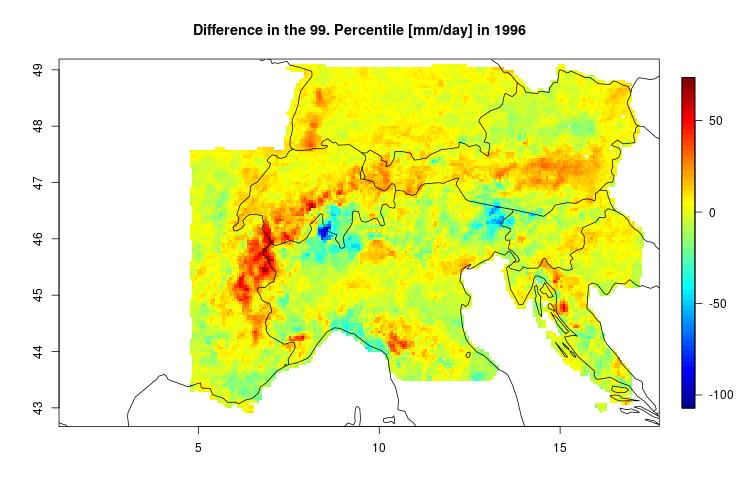
\includegraphics[width=\textwidth]{quantile_all/1996dif_q99_hist_alp3.jpg}
		\caption{Historical, ALP-3, 1996}
	\end{subfigure}
	\begin{subfigure}{0.32\textwidth}
		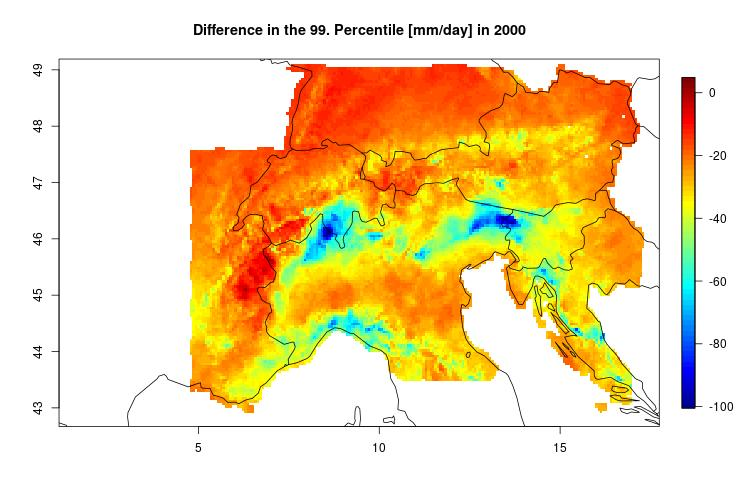
\includegraphics[width=\textwidth]{quantile_all/2000dif_q99_hist_alp3.jpg}
		\caption{Historical, ALP-3, 2000}
	\end{subfigure}
	\begin{subfigure}{0.32\textwidth}
		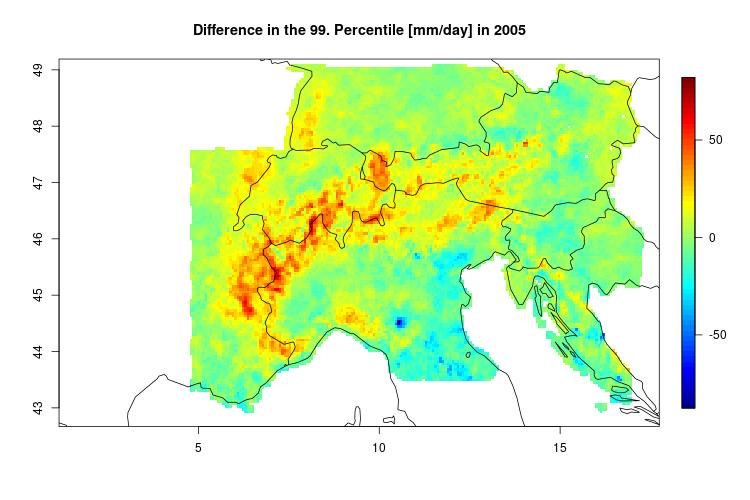
\includegraphics[width=\textwidth]{quantile_all/2005dif_q99_hist_alp3.jpg}
		\caption{Historical, ALP-3, 2005}
	\end{subfigure}
	\begin{subfigure}{0.32\textwidth}
		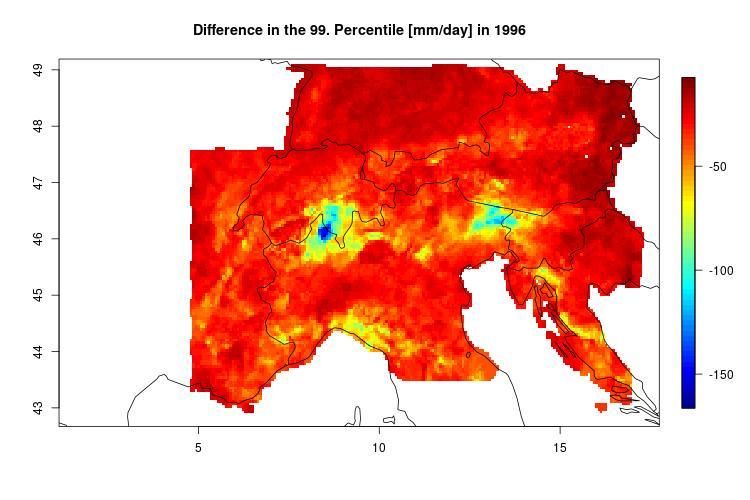
\includegraphics[width=\textwidth]{quantile_all/1996dif_q99_eval_eur11.jpg}
		\caption{Evaluation, EUR-11, 1996}
	\end{subfigure}
	\begin{subfigure}{0.32\textwidth}
		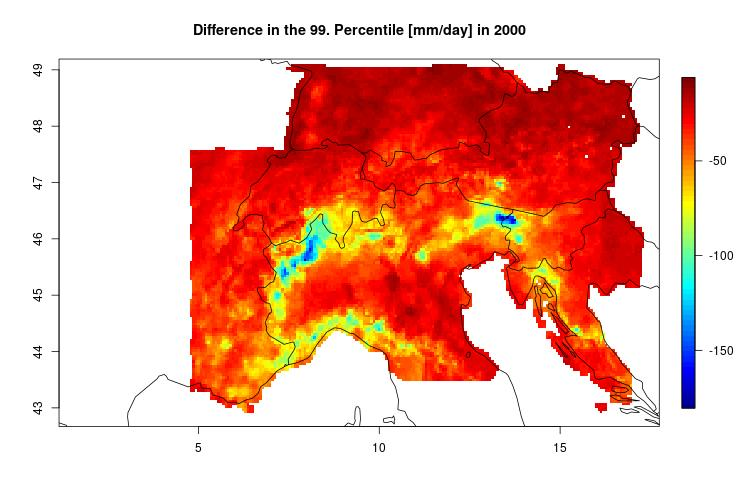
\includegraphics[width=\textwidth]{quantile_all/2000dif_q99_eval_eur11.jpg}
		\caption{Evaluation, EUR-11, 2000}
	\end{subfigure}
	\begin{subfigure}{0.32\textwidth}
		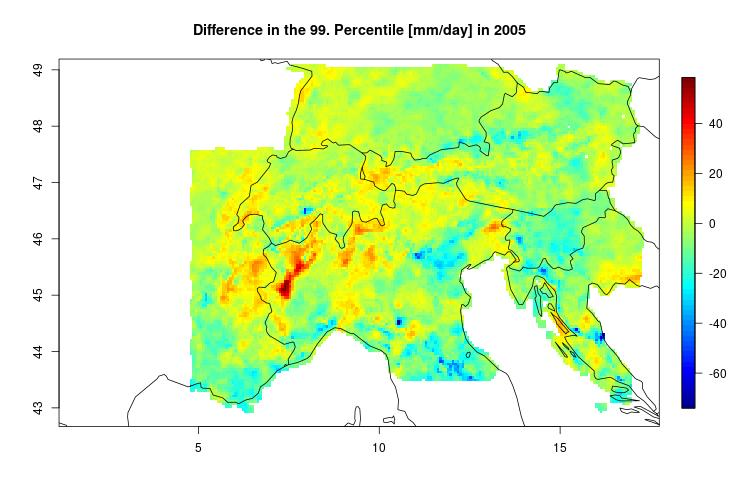
\includegraphics[width=\textwidth]{quantile_all/2005dif_q99_eval_eur11.jpg}
		\caption{Evaluation, EUR-11, 2005}
	\end{subfigure}
	\begin{subfigure}{0.32\textwidth}
		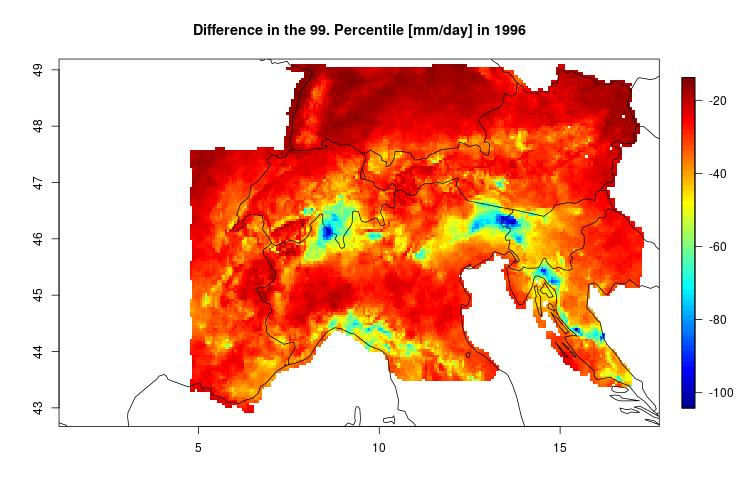
\includegraphics[width=\textwidth]{quantile_all/1996dif_q99_eval_alp3.jpg}
		\caption{Evaluation, ALP-3, 1996}
	\end{subfigure}
	\begin{subfigure}{0.32\textwidth}
		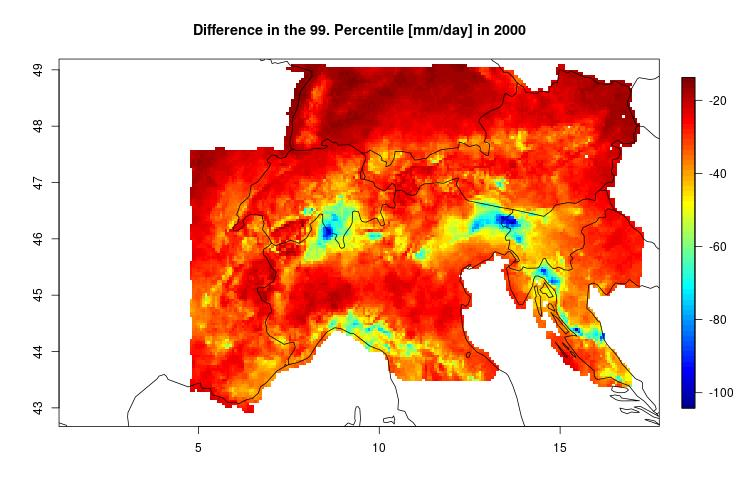
\includegraphics[width=\textwidth]{quantile_all/2000dif_q99_eval_alp3.jpg}
		\caption{Evaluation, ALP-3, 2000}
	\end{subfigure}
	\begin{subfigure}{0.32\textwidth}
		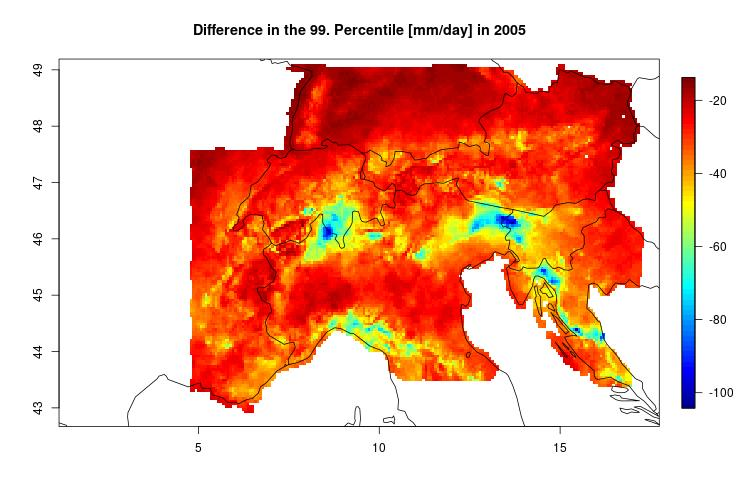
\includegraphics[width=\textwidth]{quantile_all/2005dif_q99_eval_alp3.jpg}
		\caption{Evaluation, ALP-3, 2005}
	\end{subfigure}
	\caption{Differenzen im 99.Quantil für die Jahre 1996, 2000 und 2005 (gemittelt über das Jahr)}
	\label{fig:quantile_alp3}
\end{figure}

\section{Zusammenfassung}
Da durch die in diesem Kapitel verfolgte Herangehensweise ein relativ schlechtes Ergebnis für die Vorhersage der Extremniederschläge in allen betrachteten Klimamodellen erzeugt wurde, soll im folgenden Kapitel die Extremniederschläge in den unterschiedlichen Jahreszeiten betrachtet werden. Wie in den Abbildungen \ref{fig:quantile_alp3} zu erkennen ist, scheinen manche Regionen besonders stark unterschätzte Starkregen-Ereignisse aufzuweisen. Diese Regionen wurden in ''Major flood disasters in Europe: 1950–2005'' \cite{barredo_major_2007} unter anderem als Regionen größerer Flutkatastrophen genannt. Dies weißt darauf hin, dass die Klimasimulation für solche Orte gesondert betrachtet werden muss und vielleicht von einem Klimamodell, welches den ganzen Alpenraum abdeckt nicht vollends richtig berechnet werden kann. 